\subsection{Q10.14 data 10312021 grouped by scenario \& group}

\begin{comment}
                        EFPR        EO      EFNR     n    pvalue
(frauth, majority)  0.500000  0.500000  0.375000   8.0  1.000000
(frauth, minority)  0.307692  0.692308  0.384615  13.0  0.093782
(icu, majority)     0.611111  0.388889  0.611111   9.0  0.466854
(icu, minority)     0.400000  0.600000  0.400000  10.0  0.563165
(rent, majority)    0.545455  0.454545  0.409091  11.0  0.782528
(rent, minority)    0.150000  0.850000  0.300000  10.0  0.019615
\end{comment}

\begin{table}[h]
    \centering
    \begin{tabular}{|c|c|c|c|c|c|c|}
        \hline
        scenario & group & EFPR & EO & EFNR & n & p-value\\
        \hline
        frauth & majority & 0.500 & 0.500 & 0.375 & 8.0 & 1.000\\
		frauth & minority & 0.308 & \textbf{0.692} & 0.385 & 13.0 & 0.094\\
		icu & majority & \textbf{0.611} & 0.389 & \textbf{0.611} & 9.0 & 0.467\\
		icu & minority & 0.400 & \textbf{0.600} & 0.400 & 10.0 & 0.563\\
		rent & majority & \textbf{0.545} & 0.455 & 0.409 & 11.0 & 0.783\\
		rent & minority & 0.150 & \textbf{0.850} & 0.300 & 10.0 & \textbf{0.020}\\
		
        \hline
    \end{tabular}
    \caption{Grouped by scenario group}
    \label{tab:my_label}
\end{table}
\begin{figure}[h]
    \centering
    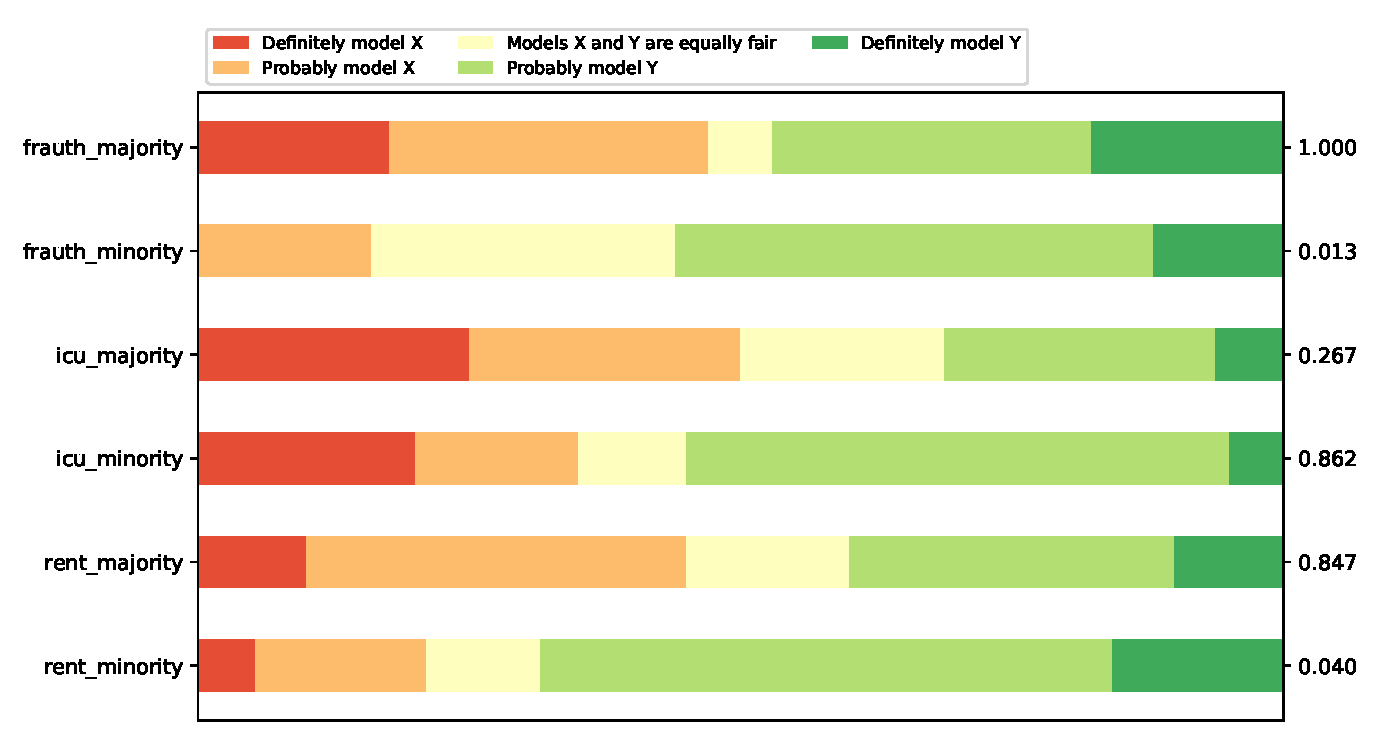
\includegraphics[width=0.8\textwidth]{figures/Q10.14/10312021/Q10.14_scenario_group.pdf}
    \caption{Grouped by scenario \& group}
    \label{fig:my_label}
\end{figure}
